% !TEX TS-program = XeLaTeX
% use the following command:
% all document files must be coded in UTF-8
\documentclass[spanish]{textolivre}
% build HTML with: make4ht -e build.lua -c textolivre.cfg -x -u article "fn-in,svg,pic-align"

\journalname{Texto Livre}
\thevolume{15}
%\thenumber{}
\theyear{2022}
\receiveddate{\DTMdisplaydate{2020}{10}{6}{-1}} % YYYY MM DD
\accepteddate{\DTMdisplaydate{2020}{11}{16}{-1}}
\publisheddate{\DTMdisplaydate{2021}{12}{15}{-1}}
\corrauthor{María-Soledad Ramírez-Montoya}
\articledoi{10.35699/1983-3652.2022.25716}
%\articleid{NNNN} % if the article ID is not the last 5 numbers of its DOI, provide it using \articleid{} commmand
% list of available sesscions in the journal: articles, dossier, reports, essays, reviews, interviews
\articlesessionname{articles}
\runningauthor{Ramírez-Montoya y González-Padrón} 
%\editorname{Leonardo Araújo}
\sectioneditorname{Daniervelin Pereira}
\layouteditorname{Anna Izabella M. Pereira}

\title{Arquitectura de horizontes en emprendimiento social: innovación con tecnologías emergentes}
\othertitle{Arquitetura de horizontes em empreendedorismo social: inovação com tecnologias emergentes}
\othertitle{Architecture of horizons in social entrepreneurship: innovation with emerging technologies}
% if there is a third language title, add here:
%\othertitle{Artikelvorlage zur Einreichung beim Texto Livre Journal}

\author[1]{María-Soledad Ramírez-Montoya \orcid{0000-0002-1274-706X} \thanks{Email: \url{solramirez@tec.mx}}}
\author[1]{José-Guadalupe González-Padrón \orcid{0000-0002-7942-744X} \thanks{Email: \url{jggonzalez@tec.mx}}}
\affil[1]{Tecnologico de Monterrey, School of Humanities and Education, Monterrey, Nuevo León, Mexico.}

\addbibresource{article.bib}
% use biber instead of bibtex
% $ biber article

% used to create dummy text for the template file
\definecolor{dark-gray}{gray}{0.35} % color used to display dummy texts
\usepackage{lipsum}
\SetLipsumParListSurrounders{\colorlet{oldcolor}{.}\color{dark-gray}}{\color{oldcolor}}

% used here only to provide the XeLaTeX and BibTeX logos
\usepackage{hologo}

% if you use multirows in a table, include the multirow package
\usepackage{multirow}

% provides sidewaysfigure environment
\usepackage{rotating}

% CUSTOM EPIGRAPH - BEGIN 
%%% https://tex.stackexchange.com/questions/193178/specific-epigraph-style
\usepackage{epigraph}
\renewcommand\textflush{flushright}
\makeatletter
\newlength\epitextskip
\pretocmd{\@epitext}{\em}{}{}
\apptocmd{\@epitext}{\em}{}{}
\patchcmd{\epigraph}{\@epitext{#1}\\}{\@epitext{#1}\\[\epitextskip]}{}{}
\makeatother
\setlength\epigraphrule{0pt}
\setlength\epitextskip{0.5ex}
\setlength\epigraphwidth{.7\textwidth}
% CUSTOM EPIGRAPH - END

% LANGUAGE - BEGIN
% ARABIC
% for languages that use special fonts, you must provide the typeface that will be used
% \setotherlanguage{arabic}
% \newfontfamily\arabicfont[Script=Arabic]{Amiri}
% \newfontfamily\arabicfontsf[Script=Arabic]{Amiri}
% \newfontfamily\arabicfonttt[Script=Arabic]{Amiri}
%
% in the article, to add arabic text use: \textlang{arabic}{ ... }
%
% RUSSIAN
% for russian text we also need to define fonts with support for Cyrillic script
% \usepackage{fontspec}
% \setotherlanguage{russian}
% \newfontfamily\cyrillicfont{Times New Roman}
% \newfontfamily\cyrillicfontsf{Times New Roman}[Script=Cyrillic]
% \newfontfamily\cyrillicfonttt{Times New Roman}[Script=Cyrillic]
%
% in the text use \begin{russian} ... \end{russian}
% LANGUAGE - END

% EMOJIS - BEGIN
% to use emoticons in your manuscript
% https://stackoverflow.com/questions/190145/how-to-insert-emoticons-in-latex/57076064
% using font Symbola, which has full support
% the font may be downloaded at:
% https://dn-works.com/ufas/
% add to preamble:
% \newfontfamily\Symbola{Symbola}
% in the text use:
% {\Symbola emojihere}
% EMOJIS - END

% LABEL REFERENCE TO DESCRIPTIVE LIST - BEGIN
% reference itens in a descriptive list using their labels instead of numbers
% insert the code below in the preambule:
%\makeatletter
%\let\orgdescriptionlabel\descriptionlabel
%\renewcommand*{\descriptionlabel}[1]{%
%  \let\orglabel\label
%  \let\label\@gobble
%  \phantomsection
%  \edef\@currentlabel{#1\unskip}%
%  \let\label\orglabel
%  \orgdescriptionlabel{#1}%
%}
%\makeatother
%
% in your document, use as illustraded here:
%\begin{description}
%  \item[first\label{itm1}] this is only an example;
%  % ...  add more items
%\end{description}
% LABEL REFERENCE TO DESCRIPTIVE LIST - END


% add line numbers for submission
%\usepackage{lineno}
%\linenumbers

\begin{document}
\maketitle

\begin{polyabstract}
\begin{abstract}
El emprendimiento social es un área importante para la formación en educación superior, donde la vinculación con diferentes sectores es estratégica para crear opciones de sustentabilidad para la ciudadanía. El objetivo de este artículo es analizar la percepción del nivel de dominio de competencias sociales por parte de estudiantes de posgrado, con un curso de diseño innovador que integró el método de Arquitectura de Horizontes, así como tecnologías emergentes (realidad virtual, aumentada, recursos abiertos y videos interactivos) para la construcción de proyectos de emprendimiento de aporte a los Objetivos de Desarrollo Sostenible. El contexto de aplicación integró estudiantes de posgrados de humanidades y educación, provenientes de 12 países de América, Europa y Asia. El curso se impartió en español, en una institución privada de México. El método de estudio fue mixto, con triangulación concurrente, donde se aplicaron escalas Likert de emprendimiento social y de innovación, así como grupos focales, a una población de 65 estudiantes, en un curso a distancia. En la escala se realizaron pruebas de hipótesis de dos colas con sigma poblacional desconocido; en los grupos focales se realizó análisis del discurso con descripciones texturales y estructurales. Los resultados dan cuenta de la percepción de la innovación educativa de tipo disruptivo en el diseño del curso y del desarrollo de la competencia de emprendimiento social, principalmente en las subcompetencias de valor social, liderazgo y personales. Este artículo puede ser de valor para estudiantes, profesores, investigadores y tomadores de decisiones, interesados en innovación educativa y emprendimiento.

\keywords{Diseño instruccional \sep Innovación educativa \sep Emprendimiento social \sep Tecnologías emergentes \sep Educación superior}
\end{abstract}

\begin{portuguese}
\begin{abstract}
O empreendedorismo social é uma área importante para a formação no ensino superior, em que a ligação com diferentes setores é estratégica para criar opções de sustentabilidade para os cidadãos. O objetivo deste artigo é analisar a percepção do nível de domínio das competências sociais por parte dos estudantes de pós-graduação, com um curso de \textit{design} inovador que integrou o método de Arquitectura de Horizontes, bem como tecnologias emergentes (realidade virtual, recursos ampliados, abertos e vídeos interactivos) para a construção de projetos empresariais que contribuam para os objetivos do desenvolvimento sustentável. O método de estudo foi misto, com triangulação simultânea, em que as escalas Likert de empreendedorismo social e inovação, bem como os grupos focais, foram aplicados a uma população de 65 estudantes, num curso de ensino a distância. Os resultados mostram a percepção de inovação educativa disruptiva na concepção do curso e o desenvolvimento da competência empresarial social, principalmente nas sub-competências de valor social, liderança e pessoal. Este artigo pode ser de valor para estudantes, professores, investigadores e decisores interessados na inovação educacional e empreendedorismo.

\keywords{Design Instrucional \sep Inovação educacional \sep Empreendedorismo Social \sep Tecnologias emergentes \sep Ensino superior}
\end{abstract}
\end{portuguese}

\begin{english}
\begin{abstract}
Social entrepreneurship is an important area for training in higher education, where the linkage with different sectors is strategic to create sustainability options for citizens. The objective of this article is to analyze the perception of the level of mastery of social skills by graduate students, with an innovative design course that integrated the method of Architecture of Horizons, as well as emerging technologies (virtual reality, augmented, open resources and interactive videos) for the construction of entrepreneurship projects that contribute to the objectives of sustainable development. The study method was mixed, with concurrent triangulation, where Likert scales of social entrepreneurship and innovation were applied, as well as focus group, to a population of 65 students, in a distance learning course. The results show the perception of disruptive educational innovation in the design of the course and the development of social entrepreneurship competence, mainly in the sub-competencies of social value, leadership and personal. This article may be of value to students, teachers, researchers, and decision makers interested in educational innovation and entrepreneurship.

\keywords{Instructional design \sep Educational innovation \sep Social entrepreneurship \sep Emerging technologies \sep Higher education}
\end{abstract}
\end{english}
% if there is another abstract, insert it here using the same scheme
\end{polyabstract}

\section{Introducción}\label{sec-intro}
En la complejidad del mundo cambiante, la incertidumbre es una constante. En las complicaciones emergentes, la formación en las instituciones de educación superior requiere crear nuevas formas que respondan a los cambios y resulta de gran valor postular por la generación de nuevas ideas que apoyen en la resolución de las problemáticas sociales.  En así como en los ambientes de aprendizaje, las finalidades que se persigan, los contenidos, los recursos tecnológicos y las estrategias son sustanciales para apoyar los procesos formativos de universitarios. 

En este marco, la formación en emprendimiento social constituye una oportunidad en las instituciones de educación superior para aportar en la resolución de problemas y crear nuevas opciones. Los procesos deben incluir experiencias de aprendizaje para los estudiantes que sean pertinentes y motivadoras, donde formar en emprendimiento no sea exclusivo de las áreas de negocios, sino que vaya más allá de la misma profesión que se estudia. En un estudio con universitarios se ubicó que la formación de la mentalidad emprendedora en los estudiantes es difícil de lograr, por lo que es necesario crear programas que se fortalezcan con la instrucción transversal en diferentes carreras \cite{portuguez-castro2020}. Desde esta perspectiva, intervenciones e investigaciones que den cuenta de los resultados son de valor para encaminar esfuerzos para promocionar este tipo de competencias con impacto en la sociedad.

En este sentido, el objetivo de este artículo es analizar la percepción del nivel de dominio de  competencias sociales por parte de estudiantes de posgrado, con un curso de diseño innovador que integró ideas conceptuales del marco Arquitectura de Horizontes \cite{barroso2019}, así como tecnologías emergentes (realidad virtual, aumentada, recursos abiertos y videos interactivos) para la construcción de proyectos de emprendimiento de aporte a los Objetivos de Desarrollo Sostenible \cite{unesco2015}. El estudio inicia presentando un sustento teórico del emprendimiento social, estrategias y tecnologías emergentes, posteriormente se plantea el método mixto que dirigió la investigación, se exponen los resultados y se cierra con conclusiones que invitan a seguir estudiando el tema.

\subsection{Emprendimiento social en ambientes universitarios}
Diversas problemáticas económicas, sociales y ambientales que enfrentamos hoy en día, pueden ser resueltas a través del emprendimiento social. Este tipo de emprendimiento representa un proceso de construcción, evaluación y búsqueda de oportunidades para realizar cambios sociales transformadores, enérgicos y dedicados \cite{utomo2019}. De igual manera, la educación tiene un impacto decisivo en la sociedad para abordar los principales desafíos y oportunidades que brinda el desarrollo sostenible \cite{sanchez-hernandez2019}, por lo que la formación en emprendimiento social podría ser  un catalizador para el logro de los Objetivos de Desarrollo Sostenible (ODS) declarados por la Organización de las Naciones Unidas (ONU), que también identifica otro elemento clave para abordar los desafíos que plantean los ODS: la innovación, entendida ésta como la generación, aceptación e implementación de nuevas ideas, procesos, productos o servicios \cite{filser2019}. Así, para conjuntar en un proceso formativo el emprendimiento social y la innovación que conlleva la resolución de ODS, es conveniente explorar diversas metodologías \emph{ad hoc}.

\subsection{Arquitectura de Horizontes para proyectos de innovación}
El desarrollo de competencias para el emprendimiento social se facilita con el diseño de escenarios de aprendizaje vivencial, a través de proyectos innovadores para la solución de problemáticas en contextos reales. Uno de lo puntos de encuentro para la generación de este tipo de experiencias son las instituciones de educación superior, quienes juegan un rol importante en esta dinámica de transformación social, ya que desde ahí se pueden vincular estrategias de emprendimiento e innovación, con un mayor impacto hacia la comunidad \cite{portuguez_castro2019}. Entre las diferentes alternativas para llegar a proponer cambios por medio del emprendimiento social, se ubica el marco de Arquitectura de Horizontes \cite{barroso2019}, concebido como un modelo adaptativo para asistir de manera cualitativa y cuantitativa nuestra capacidad de generar estrategias (toma de decisiones), emprendimientos (públicos) y futuros escenarios en sistemas complejos y de alta certidumbre, dentro de un período específico. Este modelo se desarrolla a lo largo del tiempo y a través de una complejidad simultánea integrada por los siguientes ejes:

\begin{itemize}
    \item Legado: los objetivos aspiracionales y utilitarios, así como las motivaciones de los creadores, comunidades o emprendedores. Aquí se incluyen los intereses personales, la vocación y los objetivos de las personas, las comunidades y las organizaciones dentro de un proyecto.
    \item Comunidad: análisis y mapeo de la red de personas que tienen un objetivo particular en común, un sentimiento de compañerismo como resultado de compartir actitudes, intereses y objetivos. Personas conscientes de su papel en el quehacer colectivo, especialmente en el contexto de las actividades económicas, los valores sociales y las responsabilidades cívicas.
    \item Aprendizaje: abarca las herramientas y habilidades relevantes para desarrollar, hacer crecer y gestionar proyectos individuales o colectivos. Particularmente importantes, herramientas relevantes para la economía digital y para la sostenibilidad.
    \item Tecnología: el conjunto de inversión tecnológica y conciencia para tomar las mejores decisiones, necesarias para desarrollar y sostener un proyecto en un contexto de rápido cambio tecnológico, en un marco temporal específico. 
    \item Contexto: los particulares factores socioeconómicos, políticos y ambientales en los que operan los proyectos, prestando atención a la influencia que la realidad local y las condiciones ambientales tienen en el crecimiento de los proyectos.
    \item Proyectos: una empresa individual o colaborativa que está diseñada para crear valor (social, económico, público, ambiental...), logrando un fin particular (legado).
\end{itemize}

\subsection{Innovación educativa y componentes}
Para un mejor acercamiento al área de innovación educativa, se hace una relación de los autores y temas mayormente citados en este campo durante los últimos cinco años, a través de diferentes bases de datos: Web of Science y Scopus. Uno de los primeros temas que aparece en Web of Science trata sobre el pensamiento computacional, entendido como un conjunto de habilidades de resolución de problemas que deben ser adquiridas por las nuevas generaciones de estudiantes para prosperar en un mundo digital lleno de objetos impulsados por software \cite{roman-gonzalez2017}. Los medios sociales también hacen su aparición en los temas de innovación educativa, específicamente el uso de YouTube como vehículo de enseñanza y su impacto positivo en los resultados de aprendizaje y la satisfacción de los alumnos \cite{orus2016}. Respecto a las formas de enseñanza, figura el « \emph{flip teaching} », también conocido como aula y/o enseñanza invertida, en la que se alternan las dos principales actividades del modelo tradicional: lecciones y tareas. Bajo esa metodología, ahora las lecciones se dirigen desde casa y las tareas se realizan en clase. Cabe señalar que este modelo se enriquece a través de la creación de recursos de aprendizaje generados por los mismos estudiantes \cite{fidalgo-blanco2017}. La cultura escolar no se queda fuera de los temas de innovación educativa, como lo refleja el estudio de caso de una escuela primaria australiana donde la interrupción de las estructuras escolares tradicionales colocó a los estudiantes a la vanguardia del liderazgo escolar, aunado al trabajo colaborativo entre maestros y alumnos para construir un entorno de aprendizaje democrático e inclusivo \cite{quinn2016}. Finalmente, en este primer bloque de temas relacionados con la innovación educativa, aparece una experiencia de implementación de Educación para el Desarrollo Sostenible en Alemania, donde sobresale que las ONG y los actores gubernamentales ocupan posiciones de red significativamente más centrales, prestigiosas e influyentes que las escuelas mismas \cite{kolleck2016}.

Repitiendo el ejercicio anterior, pero ahora con la base de datos Scopus, se encuentra en primer lugar un estudio sobre las variables asociadas con el rendimiento escolar en la educación superior. Los resultados destacan la estrecha relación entre la interacción social en los cursos y el rendimiento. Este aprovechamiento también está fuertemente asociado con la estimulación del aprendizaje significativo al presentar la información de manera clara, relacionarla con los estudiantes y utilizar tareas de aprendizaje conceptualmente exigentes \cite{schneider2017}. Interesante resulta la aparición de un tema relacionado con la gestión escolar: el liderazgo distribuido, el cual hace referencia al liderazgo que se comparte dentro, entre y a lo largo de las organizaciones. La aplicación de un liderazgo distribuido puede contribuir potencialmente a la mejora, transformación y cambios escolares auténticos \cite{harris2016}. Regresando al tema de las formas de enseñanza, en esta ocasión se habla del aprendizaje basado en juegos y la ludificación y/o gamificación, concretamente a través del uso de MinecraftEdu, con el que se pueden explorar las posibilidades de los entornos de aprendizaje inmersivo. Se valora positivamente el hecho de que este tipo de prácticas permiten un aprendizaje que implica un mayor nivel de actividad y compromiso por parte de los estudiantes, así como el aumento del interés y la motivación \cite{cozar-gutierrez2016}. También se vuelve a tocar el tema del aula invertida, pero ahora en el ámbito de la educación médica de posgrado, considerada en este contexto como una oportunidad para una sesión de aula más comprometida, ya que este enfoque educativo está teorizado para mejorar la participación y retención del alumno, permitiendo un aprendizaje más complejo durante la clase. Se investigan los efectos de las preguntas interactivas e interpoladas en el material de video en línea entregado para su revisión previa a la sesión de clase \cite{rose2016}. Por último, se hace referencia al fenómeno de las analíticas de aprendizaje y su interacción con los MOOC (Massive Open Online Course), proponiendo cuatro áreas de actividades: 1) la estandarización de la descripción del diseño educativo de los MOOC, 2) las instalaciones para compartir datos entre instituciones, 3) la formulación de políticas conjuntas y sus pautas éticas y, 4) enfoques de evaluación estandarizados \cite{drachsler2016}.

Al hablar de innovación educativa no solo nos referimos a un cambio en el proceso educativo, sino a diversos componentes. Para empezar, ciertamente nos podemos enfocar en un aspecto de cambio/novedad relacionado con aquellas ideas que provocan una modificación en algún aspecto de la enseñanza, pero, más allá de eso, podemos considerar un componente de valor agregado que nos lleva realmente a una mejora, beneficio o mayor calidad en todo el proceso. Aunado a lo anterior, la innovación educativa puede abordarse según su alcance, ya sea de tipo incremental o continua, sistemática, disruptiva o abierta \cite{garcia-gonzalez2019}. La innovación de tipo incremental o continua trata de cambios menores que buscan mejorar un producto, algún servicio o una tecnología; se trata de mejorar aspectos de procesos ya existentes. La innovación sistemática refiere un proceso en el que existe un análisis situacional, la definición/solución de problemas y una evaluación de las acciones realizadas. La innovación disruptiva implica cambios significativos en los procesos y suele incluir modelos complejos con productos sofisticados y/o tecnologías dominantes. Finalmente, la innovación de tipo abierta comprende la generación y transferencia de conocimiento a través de redes de colaboración tanto dentro como fuera de las organizaciones, con el objetivo de ayudar a mejorar los productos y servicios que ofrecen para ser más competitivos \cite{miranda2019}. De esta manera, la innovación educativa puede ocurrir en cualquier elemento que gira en torno a la educación, como el diseño instruccional o las prácticas actuales de los jóvenes universitarios en relación con el uso de internet, por citar algunos ejemplos.

\subsection{Diseño instruccional innovador}
Los modelos de diseño instruccional han ido evolucionando hacia nuevas formas de creación de ambientes de aprendizaje. Eso es congruente con la conceptualización del diseño que se tiene, en cuanto trata de un proceso sistemático y reflexivo que concreta los principios del aprendizaje y la enseñanza, partiendo de una planeación didáctica generalmente \cite{brown2016}. En la práctica, existen diversos modelos de diseño, resaltando entre ellos:

\begin{itemize}
    \item El modelo ADDIE. Acrónimo de Análisis, Diseño, Desarrollo, Implementación y Evaluación, que representan los componentes y/o fases de cualquier modelo de diseño instruccional y por lo que es considerado un modelo genérico \cite{dominguez_perez2018}.
    \item El modelo ASSURE. Un modelo que tiene sus bases teóricas en el constructivismo y que parte de las características del estudiante, haciéndolo protagonista de su propio aprendizaje. El acrónimo de este modelo  hace referencia a los siguientes pasos: \emph{Analize, State, Select, Utilize, Require} y \emph{Evaluate} \cite{mora2017}.
\end{itemize}

Actualmente existen nuevas tendencias en la planeación y diseño de cursos, como la que se propone desde el \emph{Learning Environment Modeling} (LEM), una herramienta de planeación visual dirigida hacia la innovación en el diseño del aprendizaje \cite{ramirez-montoya2020}. Entre sus atributos considera en el diseño los siguientes elementos:

\begin{itemize}
    \item Información: aquí se toma en cuenta el contenido que se va a proporcionar al alumno de manera unidireccional (dar  instrucciones, generar una dinámica de trabajo, temas, lecturas, videos).
    \item Diálogo: la colaboración e interacción que se pretende realizar en grupo, con el profesor, compañeros de clase o agentes externos (discusiones y debates generados en foros de discusión).
    \item \emph{Feedback}: los comentarios del profesor sobre las tareas de los alumnos, el asesoramiento y tutoría que se brinda a ellos, así como las  autoevaluaciones y evaluaciones de pares.
    \item Práctica: consiste en la realización de actividades por parte del alumno, en las que se pretende, como su nombre lo indica, poner en práctica el conocimiento adquirido (tareas, ejercicios, etc.)
    \item Evidencia: a diferencia del anterior, este elemento se enfoca más en  la obtención de una evidencia de aprendizaje: tests, pruebas finales, proyectos.
\end{itemize}

Así, con el diseño LEM se puede integrar un proceso de diseño innovador y detectar las áreas que hace falta equilibrar para alcanzar mejores resultados, por ejemplo, a través de la inclusión de algún recurso provisto con tecnologías emergentes.

\subsection{Diseño con tecnologías emergentes}
La investigación sobre el uso de tecnologías emergentes en educación refiere diversas herramientas. Por ejemplo, la realidad virtual se utiliza en una amplia gama de campos como la medicina, los juegos, la psicología y la sociología. Existen diferencias significativas en términos de “la intención de usar” y “el disfrute percibido” entre grupos que utilizan realidad virtual y los que priorizan recursos más tradicionales. Además, el uso de esta tecnología puede mejorar considerablemente las actividades de resolución de problemas en campos como la arquitectura y el diseño \cite{ozgen2021}. El uso educativo de videos digitales y otras tecnologías como \emph{software} específico para una materia, herramientas de colaboración, juegos, simulaciones y laboratorios virtuales influye en las percepciones, motivaciones y experiencias de los instructores de cursos en línea o modalidad \emph{blended learning} \cite{meletiou-mavrotheris2021}. Por otro lado, la realidad aumentada (RA) está emergiendo como una nueva tecnología en el campo de la educación en ingeniería: con la ayuda de datos 3D generados por computadora, animación, efectos visuales e inmersión, esta tecnología se ha vuelto más frecuente para facilitar la comprensión de conceptos complejos \cite{kumar2021}. La investigación en ambientes de aprendizaje y tecnologías emergentes incluye también el uso de redes sociales, MOOCs, tecnología de educación especial, aprendizaje móvil, \emph{gamification}, aprendizaje adaptativo y analíticas de aprendizaje \cite{martin2020}. En resumen, este tipo de tecnologías pueden acelerar cambios y mejoras de muchos procesos educativos, impactando significativamente en el desarrollo de competencias y resolviendo creativamente algunos problemas de la sociedad \cite{hidrogo2020}.

El diseño de un curso con tecnologías emergentes puede considerar el uso de la llamada realidad mixta: una combinación de realidad virtual (RV) y realidad aumentada (RA). La realidad virtual (RV) se refiere a la tecnología que un dispositivo o visor de realidad virtual permite al usuario teletransportarse a otros contextos virtualizados. El uso de la tecnología de realidad virtual en la educación se relaciona con los siguientes beneficios: a) facilita el aprendizaje constructivista, b) proporciona formas alternativas de aprendizaje y c) permite la colaboración entre estudiantes más allá del espacio físico. De igual manera, su uso tiene incidencia tanto en la motivación e interés de los estudiantes, como en el desarrollo de su competencia digital. Esto es propicio también en cuanto el proceso educativo requiere de comunicación y colaboración entre pares, profesores y alumnos. Por ello el interés de aplicar estas tecnologías emergentes, con el objeto de introducir contenido innovador que capte la atención y motive al estudiante en su proceso formativo. La realidad aumentada (RA) es una variación de la realidad virtual (VR), que permite al usuario ver el mundo real aumentado con objetos virtuales superpuestos. Mientras que la realidad virtual reemplaza totalmente a la realidad, la realidad aumentada la complementa, creando un entorno en el que los objetos reales/virtuales coexisten armónicamente \cite{hernandez-de-menendez2020}. El video 360° (360 grados) es otra tecnología que brinda nuevas oportunidades para el aprendizaje, dando a los estudiantes un mayor sentido de presencia. Es una alternativa viable a la realidad virtual y al video regular por su costo-beneficio y el efecto positivo en la respuesta emocional del estudiante hacia el clima de aprendizaje \cite{ulrich2021}. Cabe señalar que en el diseño del curso al cual hace referencia este artículo se han utilizado este tipo de tecnologías para favorecer el proceso de enseñanza-aprendizaje de una manera innovadora.

\section{Método}
El estudio que aquí se presenta se realizó con métodos mixtos, en diseño de triangulación concurrente \cite{onwuegbuzie2006}. Se aplicaron diversos instrumentos: escala Likert validada, pre y post \cite{garcia-gonzalez2020} para analizar las competencias de emprendimiento social; escala Likert para estudiar la percepción de innovación que los estudiantes detectaban en el curso y grupos focales con los estudiantes. El instrumento de emprendimiento social se compone de 28 indicadores que analiza cinco subcompetencias: personales, liderazgo, innovación social, valor social y gestión emprendedora. El instrumento de innovación validado \cite{garcia-gonzalez2019} se compone de 28 indicadores, estructurados en dos partes: elementos de la innovación (cambio/novedad y valor agregado) y tipos de innovación educativa (incremental, sistemática, disruptiva y abierta). Se realizaron pruebas de hipótesis de dos colas con sigma poblacional desconocido, suponiendo que su varianza es igual. El error de tipo 1 utilizado fue del 5\%. Se realizaron pruebas de hipótesis para cada una de las subcompetencias en el pretest y en el postest.

Los grupos focales analizaron las experiencias de los estudiantes respecto al dominio de la competencia, los procesos vivenciales que enfrentaron para lograr tal dominio, así como los procesos de aprendizaje que siguieron para lograrlo. Se realizó un análisis de discurso con descripciones texturales (panorama general del fenómeno de estudio a partir de los temas centrales) y estructurales (estructura de cada tema o atributos esenciales y estos pueden interpretarse en relación con los temas fenomenológicos universales). Además, de un informe general de la esencia del fenómeno (descripción compuesta enfocada en las experiencias).

Los instrumentos se aplicaron a la población de un curso sello de posgrado (Emprendimiento e innovación) del Tecnológico de Monterrey (México) que tenía por objetivo desarrollar la competencia de emprendimiento innovador a través de un proyecto integrador aplicado en un sector de impacto (gobierno, industria, academia, sociedad o medio ambiente), con el fin de aportar a los Objetivos de Desarrollo Sostenible (ODS), estipulados por la UNESCO en la agenda 2030. Fueron 65 los participantes, que cursaban estudios de Maestría en Emprendimiento Educativo, Maestría en Humanidades Digitales y Especialidad en Alta dirección de Instituciones Educativas. Los estudiantes provenían de 12 países de América, Europa y Asia. El curso se impartió en español. El período de impartición del curso se dio de enero a abril de 2020, a través de un curso a distancia que aplicó realidad virtual, aumentada, abierta y videos interactivos (\Cref{fig1}).

\begin{figure}[htbp]
 \centering
 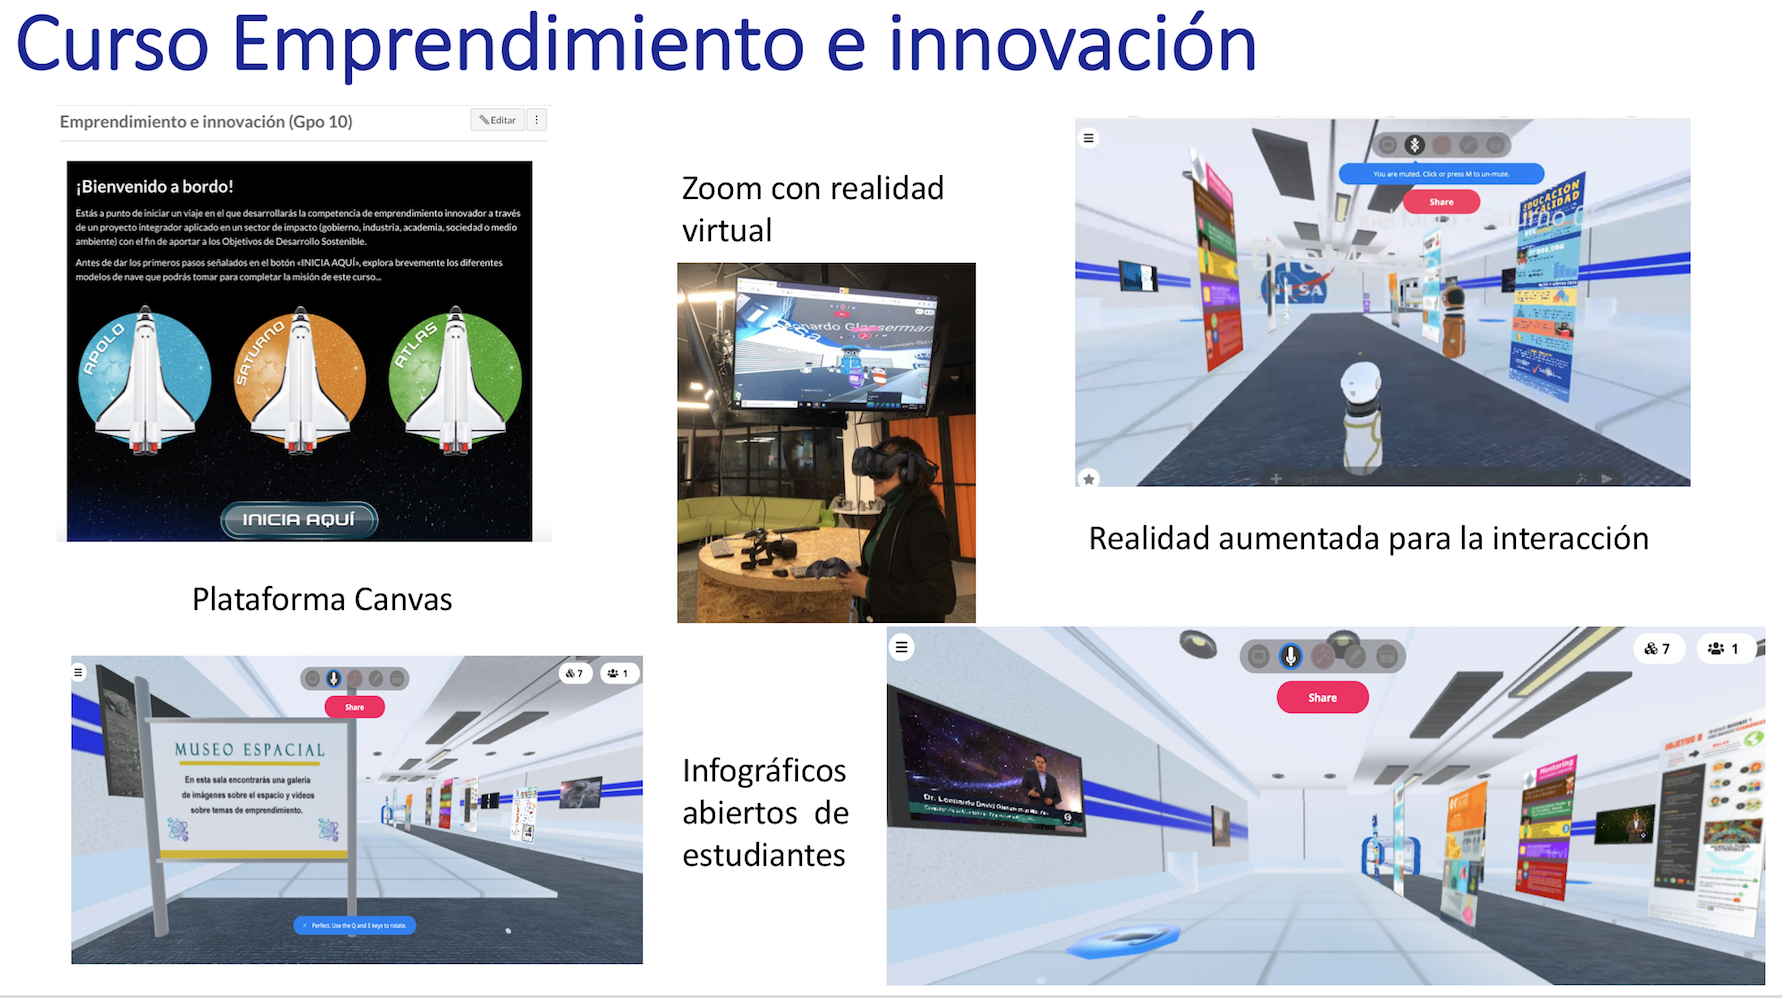
\includegraphics[width=0.7\textwidth]{fig1-25716.png}
 \caption{Imágenes del curso emprendimiento e innovación.}
 \label{fig1}
 \source{elaboración propia.}
\end{figure}

La escala likert de emprendimiento social se aplicó al inicio del curso y al final (después de cuatro meses). También se aplicó el instrumento que medía la innovación en el mes tres del curso y, finalmente, los grupos focales se aplicaron al finalizar el curso. Para el procesamiento de los datos se uso AtlasTi y análisis estadísticos con software especializado. La graficación se hizo con Tableu y Data Studio. Se realizó triangulación de datos con análisis confirmatorio, a partir de corroborar los datos obtenidos \cite{leech2007}. Los resultados se orientan a la mejora de la propuesta del modelo formativo  y se aplicaron cuestiones éticas en la investigación \cite{creswell2007, smith1990, traxler2012}, tales como información a los participantes (antes y durante la experiencia formativa), el manejo de los datos (cuidando, de manera objetiva y apegados a evidencias colectadas) y la difusión del conocimiento generado (respetando la confidencialidad de los participantes y apegada a lo que indica una entidad financiadora).

\section{Resultados}
En el entendimiento de concebir a la innovación como la integración de cambios o novedades que generan un valor agregado en la adquisición de los aprendizajes y competencias del curso, los estudiantes enunciaron que percibían que el curso aportaba un valor agregado (\Cref{fig2}).

\begin{figure}[htbp]
 \centering
 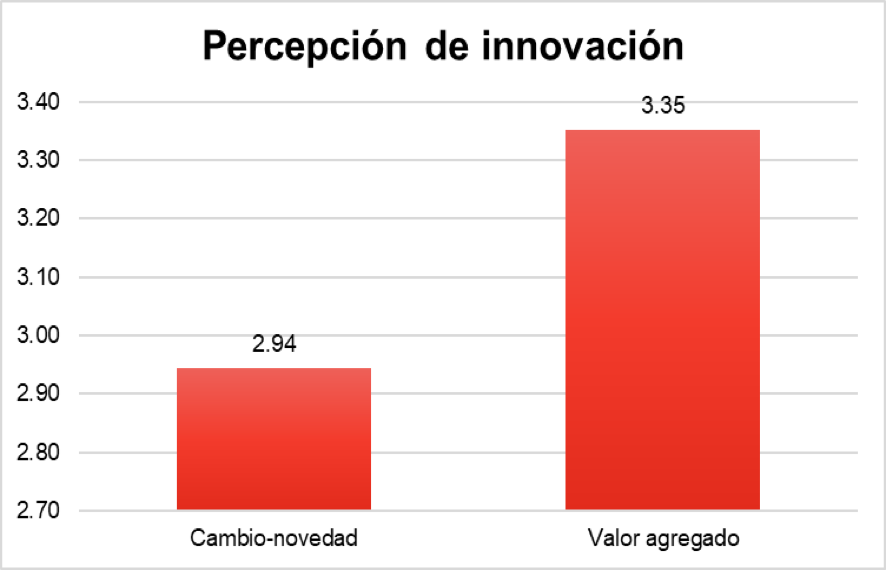
\includegraphics[width=0.6\textwidth]{fig2-25716.png}
 \caption{Percepción de innovación en el curso.}
 \label{fig2}
 \source{elaboración propia.}
\end{figure}

En el uso de las tecnologías emergentes manifestaron motivación al usar realidad virtual y aumentada, tanto en los escenarios del curso, como en los propios proyectos que ellos desarrollaron. Destaca también la metodología de Arquitectura de Horizontes y, en palabras de un estudiante: “… la arquitectura de horizontes sí es una herramienta desde mi punto de vista muy útil, para identificar problemáticas, hacer planteamientos innovadores y también clasificar el tipo de innovación, como bien dices, no tiene que ser disruptivo como en nuestro caso, que fue lo que al principio nos sacaba un poco de onda, o nos desmotivaba, porque sí queríamos sacar algo disruptivo, pero con la profundización en la investigación pues nos damos cuenta de que ya mucho se había avanzado en este tema, pero la misma arquitectura te va orientando hacia la consecución del objetivo, falta que validemos, que eso es a lo que vamos a entrar, pero siento que vamos bastante bien.” Otro equipo otorgó valor a las evaluaciones que se aplicaron en el curso: “…lo que se ha planteado para hacer el proyecto fue para mi un cambio muy enriquecedor y cómo a partir, incluso, de esa coevaluación y autoevaluación.”

En cuanto al tipo de innovación que vieron en el diseño del curso con las tecnologías emergentes integradas (relidad virtual, aumentada, videos interactivos y recursos abiertos), la distribución de las percepciones fue muy similar en los diferentes tipos, destacando la innovación disruptiva, seguida muy de cerca por la incremental y la sistémica (\Cref{fig3}).

\begin{figure}[htbp]
 \centering
 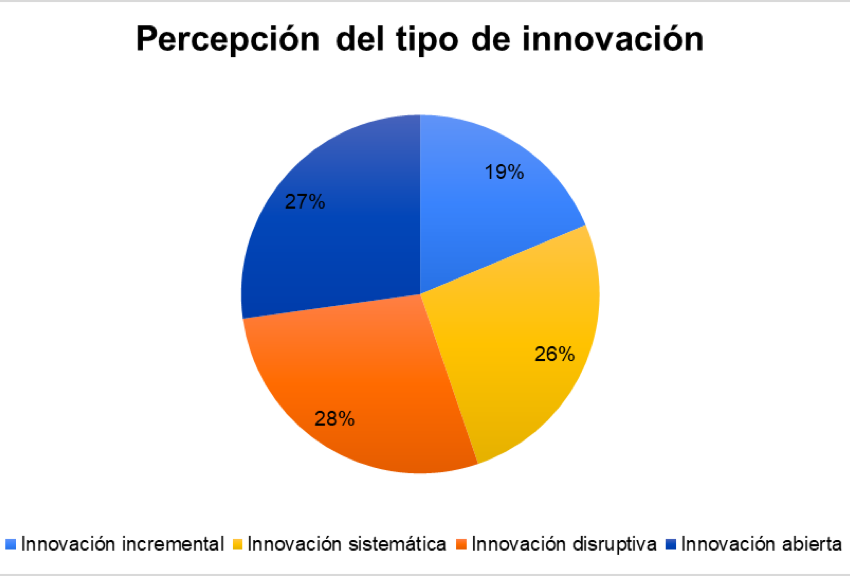
\includegraphics[width=0.6\textwidth]{fig3-25716.png}
 \caption{Percepción del tipo de innovación en el curso.}
 \label{fig3}
 \source{elaboración propia.}
\end{figure}

En el focus group los estudiantes manifestaron la novedad de trabajar con Arquitectura de Horizontes y tecnologías emergentes  en la materia, y que esto los había llevado a cuestionarse qué tan innovadores eran en sus propios planteamientos, por ejemplo, en sus propias palabras enunciaron: “…nos llegamos a preguntar sobre si nuestro proyecto era lo suficientemente innovador, porque al momento de investigar cuáles eran las tecnologías que ya se habían aplicado y algunos proyectos, pues nos dimos cuenta que ya existían algunas aplicaciones ya enfocadas a la alfabetización financiera, algunas aplicaciones desarrolladas incluso por bancos, otras pues no tenían que ver con bancos, pero estaban enfocadas en niños, y pues nos dimos cuenta, a través de la arquitectura de horizonte, que el componente innovador podría ser la aplicación de esta metodología de la enseñanza a través del juego en el sector vulnerable, porque las existentes estaban muy dirigidas hacia un sector especifico, y nuestro proyecto sí lo consideraba.”

En contraposición, en el focus group también se les preguntó a los estudiantes qué tanto sus proyectos eran innovadores y en sus palabras “… yo creo que lo principal de generar un emprendimiento social es enfocarse en resolver una problemática y no tanto en ver si es innovador o no es innovador … entonces pensando de esa manera se podría pensar qué tipo de innovación es, tal vez no estamos hablando de la innovación disruptiva, tal vez es algo incremental que está en otro contexto de manera exitosa y lo aplica a otro donde no existe. Se tendría que revisar y hacer una investigación tanto documental como con la comunidad, para ver qué tanto eso es nuevo, y qué tanto eso que se está implementando resuelve o no el problema, para que cumpla lo que es innovador.”

En el entendimiento de que el emprendimiento social es un conjunto de conocimientos, habilidades, actitudes y valores orientadas a identificar oportunidades para resolver una problemática social y/o ambiental de manera innovadora, sostenible y sistémica, transformando la realidad bajo principios éticos, los estudiantes percibieron avances en su nivel de dominio de esta competencia, desde que inició el curso (pretest) al momento que finalizó (postest) (\Cref{fig4}).

\begin{figure}[htbp]
 \centering
 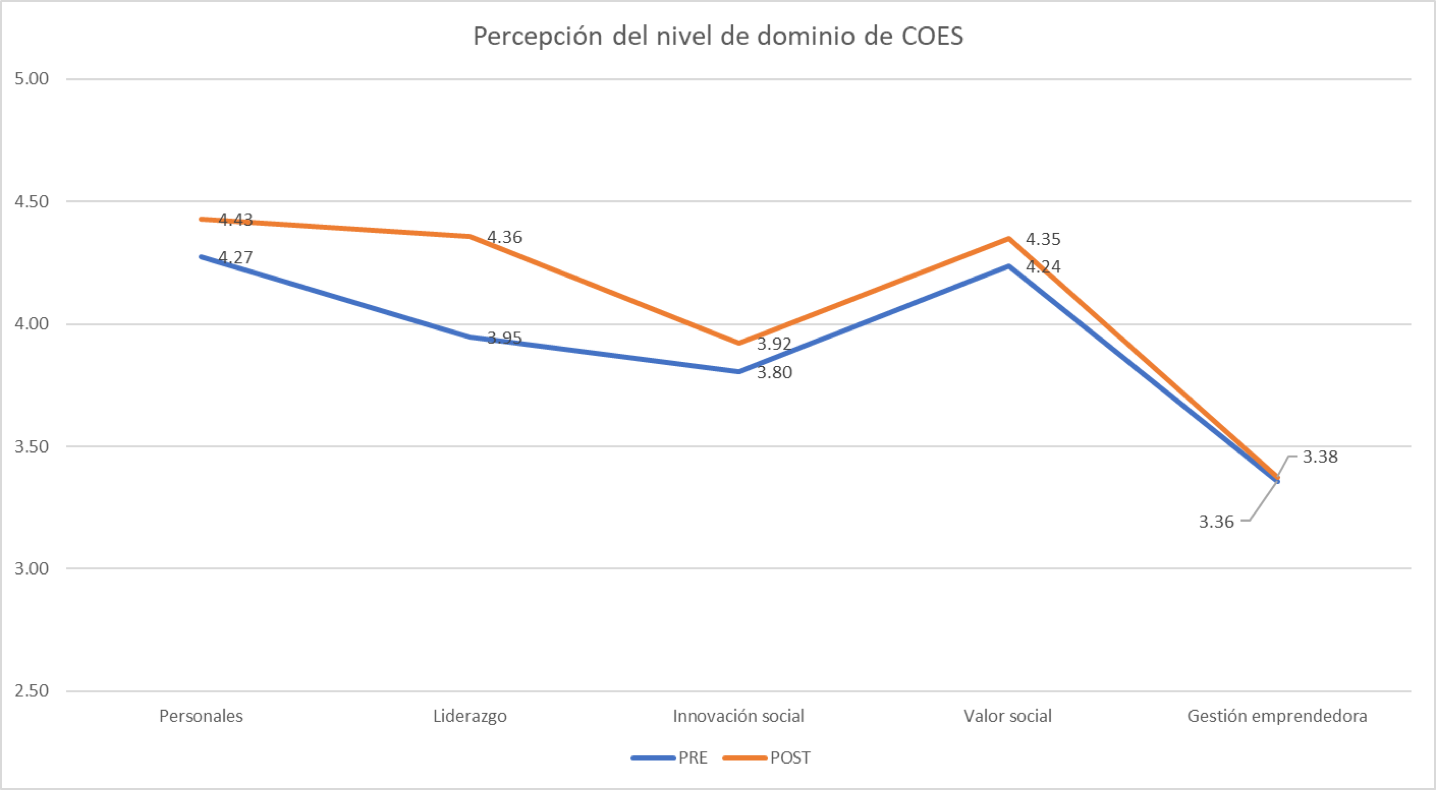
\includegraphics[width=0.8\textwidth]{fig4-25716.png}
 \caption{Percepción del nivel de dominio de las competencias sociales.}
 \label{fig4}
 \source{elaboración propia.}
\end{figure}

Fueron dos las subcompetencias de mayor nivel de dominio: liderazo y valor social, que fueron exploradas posteriormente con instrumentos cualitativos. En el focus group los estudiantes identificaron problemáticas sociales donde denotaron cualidades de liderazgo, por ejemplo “La propuesta de valor de nuestro emprendimiento, nosotros estamos viendo cómo elevar el nivel de vida de la comunidad a la que estamos proyectándonos, con base en capacitación constante y continua de los profesores de áreas rurales, que muchas veces no tienen los recursos, entonces nosotros podemos proveer de recursos e información, que ayuden a atacar esas problemáticas sociales particulares de la comunidad.”…Otro equipo enunció ”…nuestra propuesta de valor es poner mayor énfasis en educación nivel inicial, ya que la mayor sinopsis del cerebro se da en estos años, y hemos visto que los países en vías de desarrollo o subdesarrollados, seguimos con un paradigma educativa industrial, con un paradigma completamente conductista, y no hay oferta para formar a estos niños en una era post industrial, una era globalizada que requiere nuevos paradigmas educativos y nuevas estrategias de aprendizaje.”

También destacaron aportes de valor social en los proyectos que trabajaron, en sus palabras “….la propuesta de valor del emprendimiento social es, hacer un mentoring dirigido a alumnos de nivel secundaria, de pueblo originarios realizados por personas exitosas, que hayan terminado una carrera y que sea observado o cuidado por tercero que serían los mismos directos o prefectos de la institución. La problemática social que resuelve es disminuir el índice de alumnos que son de pueblos originarios, más bien, incrementar el índice de alumnos de estos pueblos que terminan la universidad.” Otro equipo manifestó “Mira, el propósito de nosotros es de derechos humanos con los alumnos de secundaria, la intención es darle curso de capacitación de docentes de manera en línea, porque en el contexto en el que estamos trabajando tenemos mucho problema de los derechos humanos, y la intención es que lo conozcan los alumnos, pero primeramente es darle la capacitación a los docentes y va a ser autoadministrable con las herramientas que se están utilizando de internet, pero empezamos con el contexto en México, somos varios países que estamos involucrados.”

En un acercamiento con las cinco subcompetencias de emprendimiento social, destacan: (a) personal, la motivación y la perseverancia; en cambio, en (b) liderazgo, resalta el trabajo colaborativo, en (c) innovación social, sobresale el aprendizaje y la adaptabilidad; en (d)  valor social, el código y sentido ético, son los más enunciados y, finalmente, en (e) gestión emprendedora, predomina el desarrollo estratégico (\Cref{fig5}).

\begin{figure}[htbp]
\centering
\begin{minipage}[t]{0.47\textwidth}
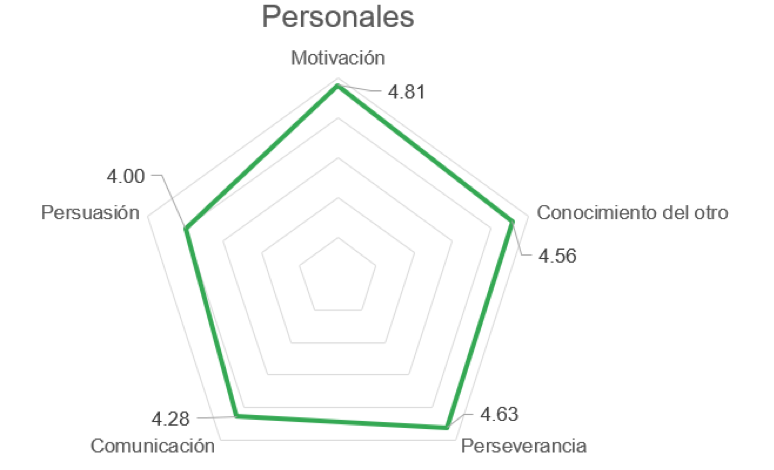
\includegraphics[width=\linewidth]{fig5-1 - 25716.png}
\subcaption{}
\end{minipage}
\hfill
\begin{minipage}[t]{0.47\textwidth}
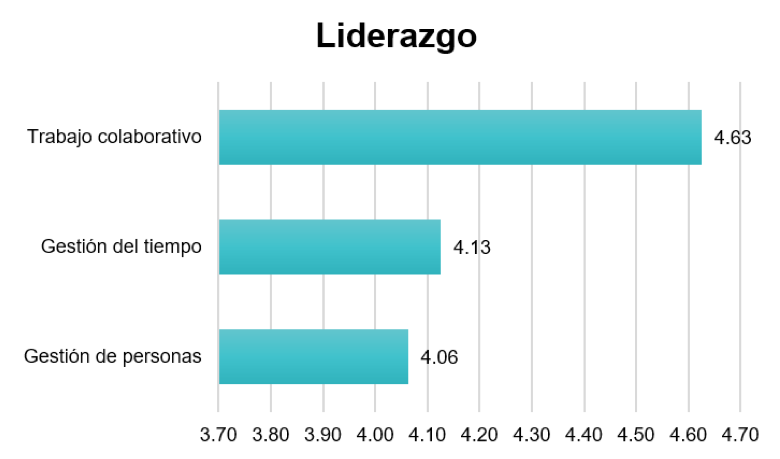
\includegraphics[width=\linewidth]{fig5-2 - 25716.png}
\subcaption{}
\end{minipage}
\hfill
\begin{minipage}[t]{0.47\textwidth}
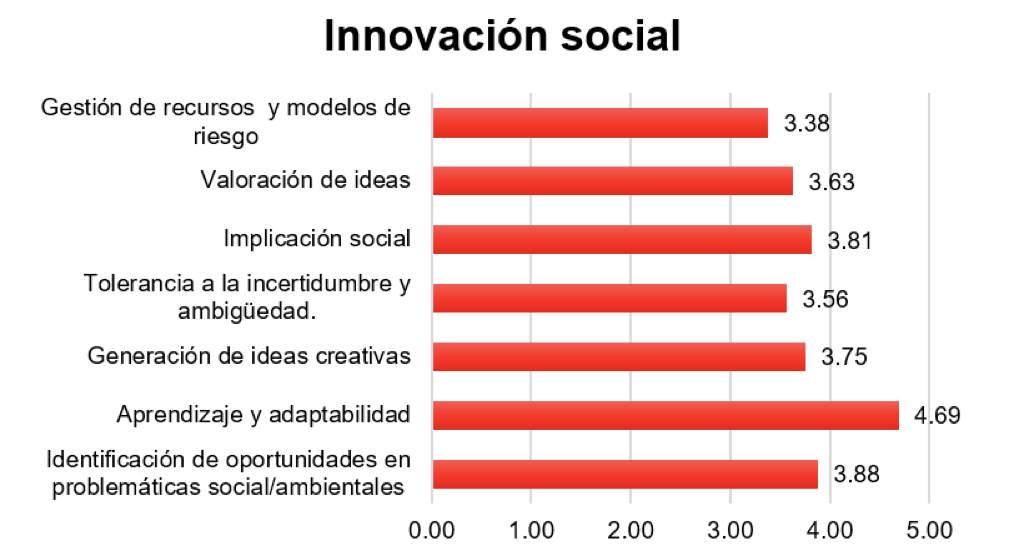
\includegraphics[width=\linewidth]{fig5-3 - 25716.png}
\subcaption{}
\end{minipage}
\hfill
\begin{minipage}[t]{0.47\textwidth}
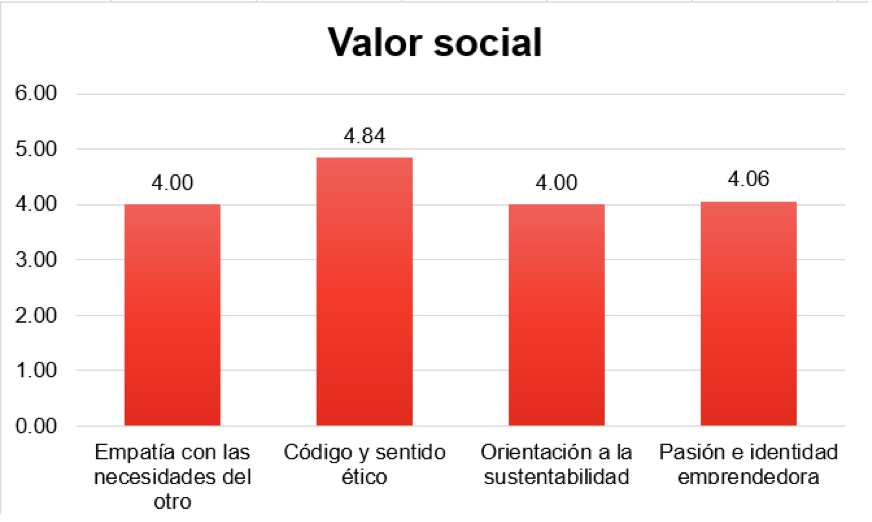
\includegraphics[width=\linewidth]{fig5-4.png}
\subcaption{}
\end{minipage}
\hfill
\begin{minipage}[t]{0.65\textwidth}
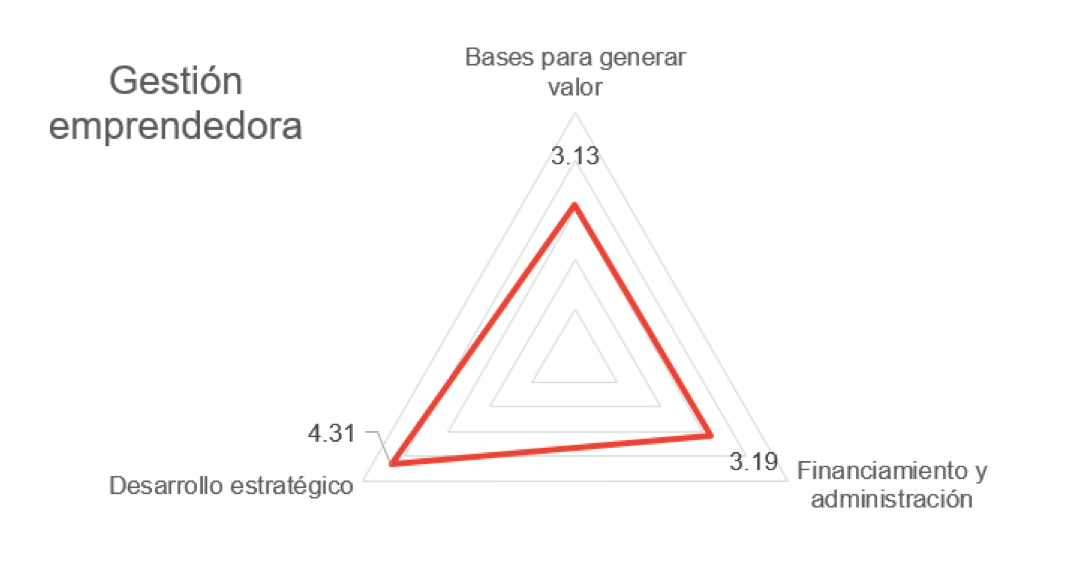
\includegraphics[width=\linewidth]{fig5-5.png}
\subcaption{}
\end{minipage}
\caption{Percepción del nivel de dominio de las competencias sociales.}
\label{fig5}
\source{elaboración propia.}
\end{figure}

En gestión emprendedora, sobresalió en el focus group el que los estudiantes denotaban bases para generar valor, en sus palabras “Nuestra propuesta de valor consiste en ampliar la alfabetización financiera para los sectores vulnerables a través de herramientas y técnicas de gamificación, y lo que pretendemos es contribuir a disminuir las desigualdades según los ODS.” Otro equipo también enunció “…nuestro proyecto antes que nada se denomina Tequio, que es una práctica comunitaria de las comunidades indígenas de México, y en nuestra propuesta de valor, es conectar a los niños de primaria de una escuela rural con una de la urbe, y a partir de ahí pues acortar esa brecha para digamos, atacar la problemática del medio ambiente que entre estos dos grupos tengan una interacción para poder resolver o generar ideas sustentables para el futuro.” 

El trabajo colaborativo y el valor de las redes fueron componentes muy mencionados en el focus group de los estudiantes, algunos ejemplos enunciados son los siguientes: “…en nuestro equipo, tenemos la intención de trabajar con los maestros de poblaciones rurales, y por ejemplo, muchos de nuestros miembros, de hecho, varios de nuestros miembros son de distintos estados que laboran en lugares así, entonces ahí sería establecer esas redes en las mismas escuelas en las que queremos trabajar, o sería buscar en organismos nacionales que ya hayan trabajado en esas comunidades o con las mismas comunidades directamente. Es lo que estamos pensando.” Otro equipo también enunció ideas de colaboración para el proyecto “…nosotros hemos puesto satélites colaboradores….En este caso del sistema de gobierno en México y de Bolivia tendrán que abrirse a algo más, porque tienen que seguir un curriculo, y después el apoyo de instituciones con alto reconocimiento al nivel mundial como el Tec de Monterrey, que innove no solamente de la educación, sino en brindar apoyo para dar a conocer la importancia de la educación en esta etapa, en esta primera etapa \emph{pues eeh}, en eso estamos.” 

Por el contrario, otro equipo reconoció que, en un principio, no habían pensado en las redes, pero tuvieron un cambio de aprendizaje y adaptabilidad de sus ideas: “…Nosotros no planteamos desde el principio en establecer redes de colaboración, pero en el camino nos hemos dado cuenta de que hay algunas otras instituciones que persiguen objetivos similares, entonces para poder establecer estas redes tendríamos que hacer esta búsqueda de organismos, ya sea, instituciones públicas o privadas que busquen de alguna manera este tipo de objetivos y establecer contacto y trabajar en conjunto, por ejemplo que si nosotros estamos buscando alfabetización financiera, educación financiera, bueno, hay muchos organismos públicos que tienen ese fin, pero también otros, como las cajas populares, que son sociedades cooperativas que también tienen dentro de sus actividades la alfabetización, aunque ellos lo hacen exclusivamente con socios, se podría establecer alguna especie de colaboración utilizando la infraestructura que ellos ya tienen montada para llegar a gente, aun cuando no sean socios, sería a través de identificar estos objetivos comunes ¿no?, pienso.”

En aspectos de liderazgo los estudiantes reconocieron que el trabajo colaborativo y la gestión de tiempos son importantes, en sus palabras “…Hay un gran reto para nosotros para establecer las redes de colaboración del proyecto, porque, finalmente, recabar toda una base de datos de posibles mentores para nuestros alumnos, va a ser un poco difícil para encontrar qué es aquello que va a mover precisamente al profesionista, para apoyar a estos alumnos. Sabemos que la parte aquí difícil es el tiempo, el tiempo de los profesionistas, optimizar el tiempo, mediante el uso de la tecnología tal vez, sí lo hemos comentado con algunos compañeros, es ir a los diferentes colegios de profesionistas y solicitar precisamente con ellos su tiempo y la orientación a un niño para que pueda aspirar, llegar inclusive a educación superior. Entonces, sí es un reto, porque es la parte básica de nuestro proyecto, establecer una red colaboración para tener un número definidos de mentores para nuestros alumnos.” También otro equipo enunció estos dos elementos (trabajo colaborativo y gestión del tiempo, en sus propios aprendizajes “…sí, en nuestro equipo se hizo todo el proyecto, fue mucho lo de la investigación, pero sobre todo la metodología que utilizamos fue el darnos las tareas, todos los del equipo, y hacer una planeación de lo que queríamos en, aunque tuvimos varias líneas de investigación, al final sí se desarrolló con base en un solo centro de trabajo; después del apoyo y todo lo que investigamos y la asesoría que nos daban las tutoras, pero sí la metodología fue la buena organización que tuvimos y bien claro el objetivo de lo que queríamos hacer, sí nos funcionó.”

La gestión emprendedora y ubicar un objetivo compartido fue clave para desarrollar sus proyecto, en palabras de un estudiante “… en nuestro caso, vimos que nuestra visión era algo ambiciosa, entonces, tenemos miembros del equipo en San Luis, Monterrey, Nayarit, como que queríamos abarcar todos los contextos. Por lo que lo primero que reflexionamos fue que tenemos que acotarnos para lograr definirnos, ya después podemos volver a expandirnos y crecer a otros, entonces, en base a todos los contextos que teníamos, teníamos que ver, qué características teníamos en común, y con base en eso, desarrollarnos más claro más a detalle, para tener una idea, de ok, vamos a trabajar en comunidades rurales, entonces ahí el aprendizaje en esa parte fue acotar el objetivo, qué es lo que vas a trabajar primero y hacerlo bien.” Otro equipo también indicó la importancia de una identificación compartida “….sí, nosotros en cuanto a experiencia y haría énfasis, en la parte de identificar bien el problema y plantear la posible solución, \emph{eh}, la dificultad en la identificación del problema nos llevó a cambiar la idea original, justo unos días antes de la primera entrega, porque nosotros estábamos, pensando en la comunidad migrante y como ellos podían construir un tipo de red para bajar los costos del envío y recepción de remesas, y esto fue porque no teníamos claridad en cuanto al conocimiento del tema, entonces por eso hacer énfasis en la parte de la investigación como una fase previa para identificar el problema y plantear una solución, que eso fue lo que nos ayudó a salir adelante, el profundizar en lo que tenía que ver con educación financiera, sí es lo que teníamos claro desde el principio, que era lo que queríamos incidir, y bueno, el desconocimiento en el acceso a fuentes de información actualizado, que al final del día sí lo pudimos también resolver, eso es lo que yo hablaría sobre nuestra experiencia.”

Otorgar valor fue un elemento compartido en los diferentes proyectos de los estudiantes, por ejemplo, un equipo enunció “… Bueno, el proyecto de mi equipo, se enfoca en trabajo decente del ODS 8 que es trabajo decente y desarrollo económico y va hacia la meta 8.9 que va con turismo sostenible….nosotros estamos en trabajo del área del turismo sostenible, que es el área en que ninguno de los tres integrantes del equipo tiene mucha experiencia, yo creo que ese podría ser un reto para este equipo y bueno, el legado, lo que queremos, lo que pretendemos con el proyecto es llegar o llevar a las comunidades o la comunidad de Creel, que es un pueblo mágico que se encuentra en Chihuahua el llegar a Creel con una propuesta de incorporar agricultura vertical como una manera de producir el cultivos, variados en este pueblo, con la intención de que estos cultivos variados generen de pronto  una propuesta gastronómica para los turistas que visitan esta área y también pues sería la otra intención que este tipo de agricultura generara posibilidades de empleo decente sobre todo para las mujeres que habitan este pueblo, esa es como la propuesta que nosotros tenemos para el proyecto.”

Un aspecto que salió bajo en los resultados fue el tema del financiamiento y la administración, de hecho, en el marco de Arquitectura de horizontes no se contempló y los alumnos enunciaron esta ausencia “… quizá para el desarrollo del proyecto que hablamos de cómo establecer relaciones y todo eso, no nos habíamos puesto a pensar en el financiamiento de dónde vamos a tener recursos para echar a andar el proyecto, hasta ahorita lo hacemos con mucho corazón. Sí, es algo muy importante que no lo habíamos considerado.” Y otro equipo canalizó el aspecto financiero hacia otras dependencias “…bueno pues, nosotros ya hemos contemplado esa parte más, estamos empalmando otras teorías que puedan suceder, por ejemplo, la responsabilidad social empresarial de otras empresas y las fundaciones que aunque vamos a ser autosustentables, o sea, un social bussines, eeh, una ventaja tenemos que somos países en vías de desarrollo entonces, las fundaciones siempre pueden ser una buena fuente no solo de recursos económicos, sino de capital humano, transferencia de información de know how, y del benchmarking que se podría obtener de ellos, aunque nuestra instituciones es completamente nueva porque no es que queremos que nos regalen la plata, pero sí que nos den un capital semilla, pero no 3 mil dólares, porque con 3 mil dólares pues no haces nada, porque eso es como un regalo y ya se ha demostrado económicamente que eso es obsoleto, sino que nos den un buen financiamiento para poder iniciar el proyecto, y un buen plan de pagos en el cual podemos a ellos retribuirles por el préstamos para pagarles a ellos. Y esto es un ganar-ganar, porque ellos tienen que cumplir por un lado responsabilidad social empresarial y nosotros queremos enfocarnos en el tema de la educación, entonces en eso vamos.”

\section{Conclusiones}
El objetivo de este artículo se ubicó en el análisis de la percepción del nivel de dominio de competencias sociales por parte de estudiantes de posgrado, con un curso de diseño innovador que integró el método de Arquitectura de Horizontes, así como tecnologías emergentes (realidad virtual, aumentada, recursos abiertos y videos interactivos) para la construcción de proyectos de emprendimiento de aporte a los Objetivos de Desarrollo Sostenible. Los resultados dieron cuenta de la percepción de la innovación educativa de tipo disruptivo en el diseño del curso y del desarrollo de la competencia de emprendimiento social, principalmente en las subcompetencias de valor social, liderazgo y personales.

La innovación educativa pasa por contemplar nuevos procesos y productos que pueden ser integrados a través de diseños, estrategias metodológicas y recursos que apoyen en la mejora de los aprendizajes y que sean reconocidos por los participantes de una instancia formativa. En el caso presentado, la \Cref{fig1} da cuenta de las innovaciones integradas y las \Cref{fig2,fig3} enuncian el reconocimiento de los estudiantes hacia el reconocimiento de valor agregado e innovación disruptiva. La innovación disruptiva implica cambios significativos en los procesos y suele incluir modelos complejos con productos y/o tecnologías \cite{garcia-gonzalez2019}. Buscar mejoras en los aprendizajes de los estudiantes postula por integrar nuevas opciones en el proceso formativo que apueste por el cambio.

Escalar niveles de dominio en competencias sociales refleja compromiso con problemáticas con aporte de valor social, actitudes de liderazgo y personales. En las \Cref{fig4,fig5} se reflejan el incremento en el dominio, desde la percepción de los estudiantes, además de que en el focus group se manifestaron las ideas para gestar proyectos que otorgaran valor a la sociedad. El emprendimiento representa un proceso de construcción, evaluación y búsqueda de oportunidades para realizar cambios sociales transformadores \cite{utomo2019}, donde la formación puede tener un impacto decisivo en la sociedad para abordar los principales desafíos y oportunidades que brinda el desarrollo sostenible \cite{sanchez-hernandez2019}. Postular por una formación en emprendimiento social llevará a generar nuevas oportunidades para la creación de soluciones sustentables.

Desde la concepción del curso se tuvo la consigna de permear elementos de innovación en todos los aspectos y tareas a realizar para producir el curso en línea que aquí se refiere. Y así fue. En el proceso de diseño se implementó la planeación visual que el modelo de ambientes de aprendizaje (LEM) conlleva, tomando decisiones que, a la postre, tuvieron su impacto en los resultados positivos que se obtuvieron durante la investigación. Entre esas decisiones resaltan la adopción del marco de Arquitectura de Horizontes para abordar los contenidos de emprendimiento e innovación, que configuran la materia del curso. Asimismo, el uso de tecnologías emergentes como la realidad virtual y la realidad aumentada, además de los videos interactivos y los recursos abiertos, han incidido positivamente en la percepción de innovación que los alumnos han manifestado.

No hay que dejar de lado otro gran eje conductor de la experiencia de aprendizaje que desde el diseño del curso se enfatizó: la formación de emprendimiento social. Algo que satisfactoriamente se fue desarrollando y reflejando también de manera favorable en los niveles de dominio que expresaron los alumnos a quienes se dirigieron estos esfuerzos. Con los resultados del estudio se pudieron detectar las subcompetencias que se desarrollaron con mayor énfasis (subcompetencias de valor social, liderazgo y personales) e incluso aquellas donde no se llegó a obtener incrementos en el nivel de dominio (gestión financiera), lo que da lugar a integrar mejoras en nuevas ediciones en que se trabaje con el marco de Arquitectura de Horizontes.

Entre las limitaciones de este estudio se puede enunciar que el curso llega a la validación de proyectos innovadores, quedando una tarea pendiente para dar seguimiento posteriormente y conocer resultados concretos de los emprendimientos sociales. Otra área de oportunidad es integrar el componente de Gestión emprendedora en la dinámica de Arquitectura de Horizontes y estudiar si la inclusión produce un incremento en esta subcompetencia que salió más baja.

Finalmente y sin lugar a dudas, el hecho de adoptar procesos y elementos innovadores en la construcción, implementación y vivencia de estos ambientes de aprendizaje, así como tecnologías emergentes, permiten el logro de ese valor agregado que nos irá llevando cada vez más a seguir transformando y diseñando mejores experiencias educativas de aporte a la visualización de nuevas creaciones. Queda con este escrito una invitación para seguir impulsando mejoras en búsqueda de contribuir con la formación de estudiantes que trasciendan a través de sus acciones y compromiso con la sociedad.

\section*{Reconocimiento}
Esta publicación es producto del proyecto “OpenSocialLab: vinculación con aprendizaje vivencial para escalar niveles de dominio en competencias de emprendimiento social”, con financiamiento del Fondo NOVUS 2019. Se agradece el apoyo del Tecnológico de Monterrey para los proyectos de innovación educativa (Convenio: Novus 2019) y a los participantes del curso por sus aportaciones para este estudio.


\printbibliography\label{sec-bib}
% if the text is not in Portuguese, it might be necessary to use the code below instead to print the correct ABNT abbreviations [s.n.], [s.l.]
%\begin{portuguese}
%\printbibliography[title={Bibliography}]
%\end{portuguese}


%full list: conceptualization,datacuration,formalanalysis,funding,investigation,methodology,projadm,resources,software,supervision,validation,visualization,writing,review
\begin{contributors}[sec-contributors]
\authorcontribution{María-Soledad Ramírez-Montoya}[projadm,funding,investigation,methodology,writing,supervision,validation,visualization,review]
\authorcontribution{José-Guadalupe González-Padrón}[formalanalysis,conceptualization,datacuration,resources,software,review]
\end{contributors}

\end{document}
